

\begin{table}[H]
\begin{flushleft}\emph{\textbf{Use Case}}\end{flushleft}
\footnotesize
\centering
\settowidth\tymin{\textbf{Entry conditions}}
\setlength\extrarowheight{2pt}
\begin{tabulary}{\textwidth}{|J|J|}
\hline
Name             & Register and Verify account \\
\hline 
Actor            & Unregistered User \\
\hline 
Entry conditions & User installed the App successfully on the proper device (which has GPS and Camera, also appropriate OS) with access to the Internet and enough storage space.\\
\hline 
Events flow      & 
\begin{minipage}[t]{0.6\textwidth}
\begin{enumerate} 
\item User opens the App and sees the welcome pages 
\item by skipping the welcome pages, the user will see the login and registration page then he/she could move to the registration part
\item In the registration part, the user will fill up the mandatory fields and if the user wants could also   fill optional fields; next by checking the box related to "terms of service" the data will be sent to the system.
\item The user should wait for the SMS from the system which contains a code in it and enters the code; in the next section, she/he should verify the email address used for registration. Eventually, the registration process will be finished after email verification.
\end{enumerate}
\end{minipage}\\
\hline
Exit conditions  & The User will see the successful registration page and will be driven to the Login page.\\
\hline
Exceptions       & 
\begin{minipage}[t]{0.6\textwidth}
\begin{itemize} 
\item Not enough storage space: showing a warning to the user which there is not enough space to could cache  needed files.
\item No Internet connection: Showing an Error message which says to continue the process the Internet   connection is necessary.
\item Duplicate username: Showing an Error message to the user to change the username or if he/sheforgot the password it could be recovered by linking to the related part of the App.
\item Improper username or ignoring the constraints in the form:showing an Error message to the user before he/she could check the "terms of service" box.
\item Not receiving the SMS of verification: showing Warning after the timer of this section finished which tells the user to continue the process the new message should be requested. If the number of requests becomes more than 10 then display an Error message to the user to begin the registration process from the beginning and drivethe user to the Welcome pages.
\item Not receiving the email of verfication: display warning which email is not verified and if there is no email in inbox or spam box, request for the new verification email. If the number of requests becomes more than 15 then display an Error message to the user to begin the registration process from the beginning and drive the user to the Welcome pages.
\item Not checking the "terms of service" box: display Warning which accepting the terms of service is vital for registration.
\item Any problem from the system: display an Error and apologies from the user and ask for another try in future
\item Any software bug in the application: display an Error message and ask from the user to send the log of the crash to the system and close the App
\end{itemize}
\end{minipage}\\
\hline
\end{tabulary}
\caption{\label{tab:Register-Verify-account}Registeration and Verifiction of account usecase}
\end{table}

The following diagrams, describe the registration process in terms of activity and runtime diagrams. The process is constituted by the filling and submission of the registration form, after which, the user receives email and SMS verification. If confirmed, the registration process is complete.

\begin{figure}[H]
\begin{flushleft}\emph{\textbf{Activity Diagram}}\end{flushleft}
\caption{Activity Diagram for Registration and Verification}
\label{register-verify-AD}
\centering
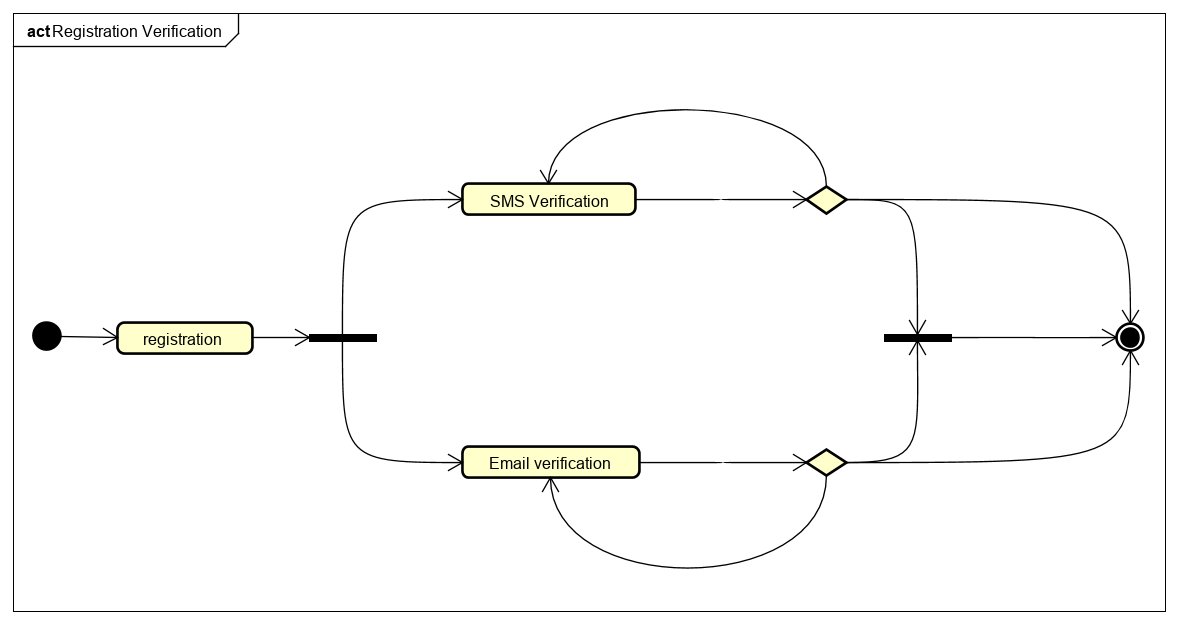
\includegraphics[width=\textwidth, height=0.50\textheight]{register-verify-AD.png}
\end{figure}
%***place holder for registration-ad***

\begin{figure}[H]
\begin{flushleft}\emph{\textbf{Sequence Diagram}}\end{flushleft}
\caption{Sequence Diagram for Registration and Verification}
\label{fig:register-verify-SD}
\centering
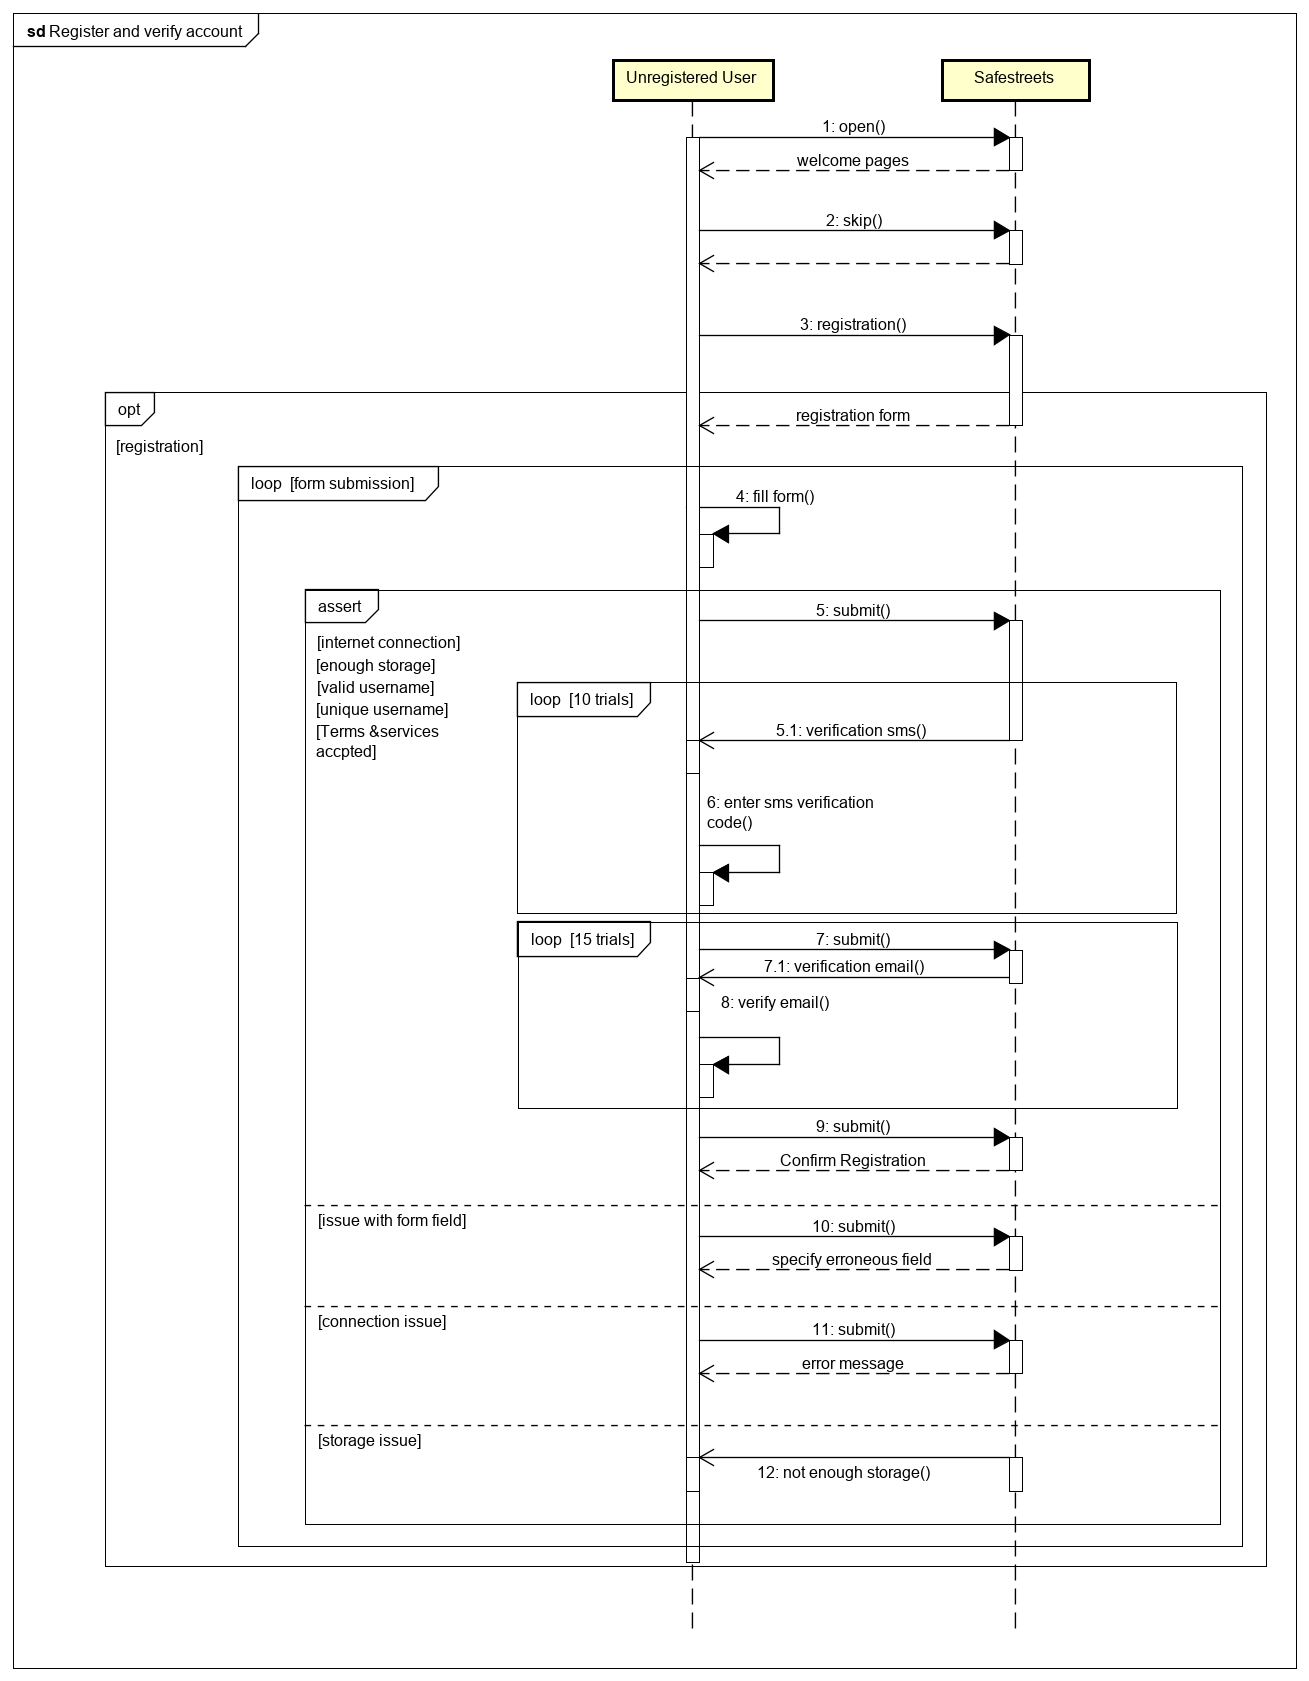
\includegraphics[width=\textwidth, height=0.90\textheight]{register-verify-SD.png}
\end{figure}
%***place holder for registration-sd***

\paragraph{Login}
\hfill \break

\begin{table}[H]
\begin{flushleft}\emph{\textbf{Use Case}}\end{flushleft}
\footnotesize
\centering
\settowidth\tymin{\textbf{Entry conditions}}
\setlength\extrarowheight{2pt}
\begin{tabulary}{\textwidth}{|J|J|}
\hline
Name             & Login \\
\hline
Actor            & Registered User \\
\hline
Entry conditions & The User should have a verified account in the system and installed App in a proper device (which has GPS and Camera, also appropriate OS) with access to the Internet and enough storage space.\\
\hline 
Events flow      & The user will open the App and enters the credentials for login and if she/he wants to speed up the reporting violation and not logging in to the app every time, the user will check the "keep me logged in" box. If the credentials are valid the user will be driven to the reporting violation page.\\
\hline 
Exit conditions  & The user successfully login to the application.\\
\hline 
Exceptions       & 
\begin{minipage}[t]{0.8\textwidth}
\begin{itemize} 
\item Absence of user name: display a warning page in which the entered username does not exist and gives an option to the user to be driven to the registration section.
\item Incorrect Credential: show an Error message to the user in which the entered credential is wrong.
\item Not enough storage space: showing a warning to the user which there is not enough space to could cache needed files.
\item No Internet connection: Showing an Error message which says to continue the process the Internet connection is necessary.
\item Any problem from the system: display an Error and apologies from the user and ask for another try in future
\item Any software bug in the application: display an Error message and ask from the user to send the log of the crash to the system and close the app
\end{itemize}
\end{minipage}\\
\hline
\end{tabulary}
\caption{\label{tab:Usecase-Login}Usecase for Login}
\end{table}

The login process is shown in the following figures. The user starts by submitting their login credentials. The system then checks them, and if verified the user is redirected to the homepage of the application. If however, there are issues with the credentials the user is notified and allowed to try again with a maximum of 20 trials.

\begin{figure}[H]
\begin{flushleft}\emph{\textbf{Activity Diagram}}\end{flushleft}
\caption{Activity Diagram for Login}
\label{fig:AD-login}
\centering
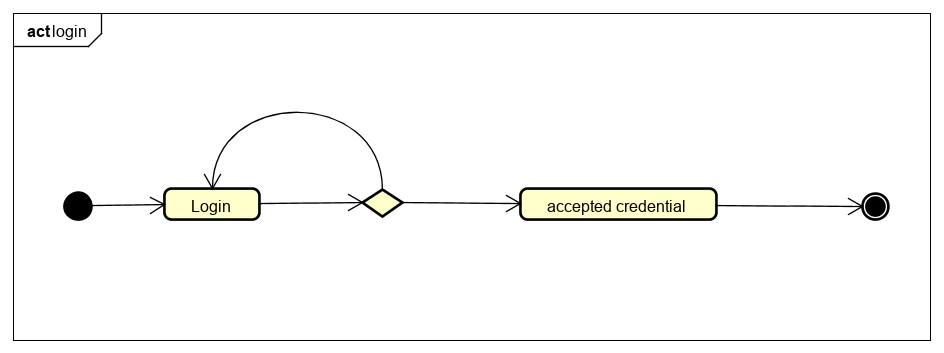
\includegraphics[width=0.7\textwidth, height=0.3\textheight]{login-AD.png}
\end{figure}
%***place holder for login-ad***

\begin{figure}[H]
\begin{flushleft}\emph{\textbf{Sequence Diagram}}\end{flushleft}
\caption{Sequence Diagram for Login}
\label{fig:SD-login}
\centering
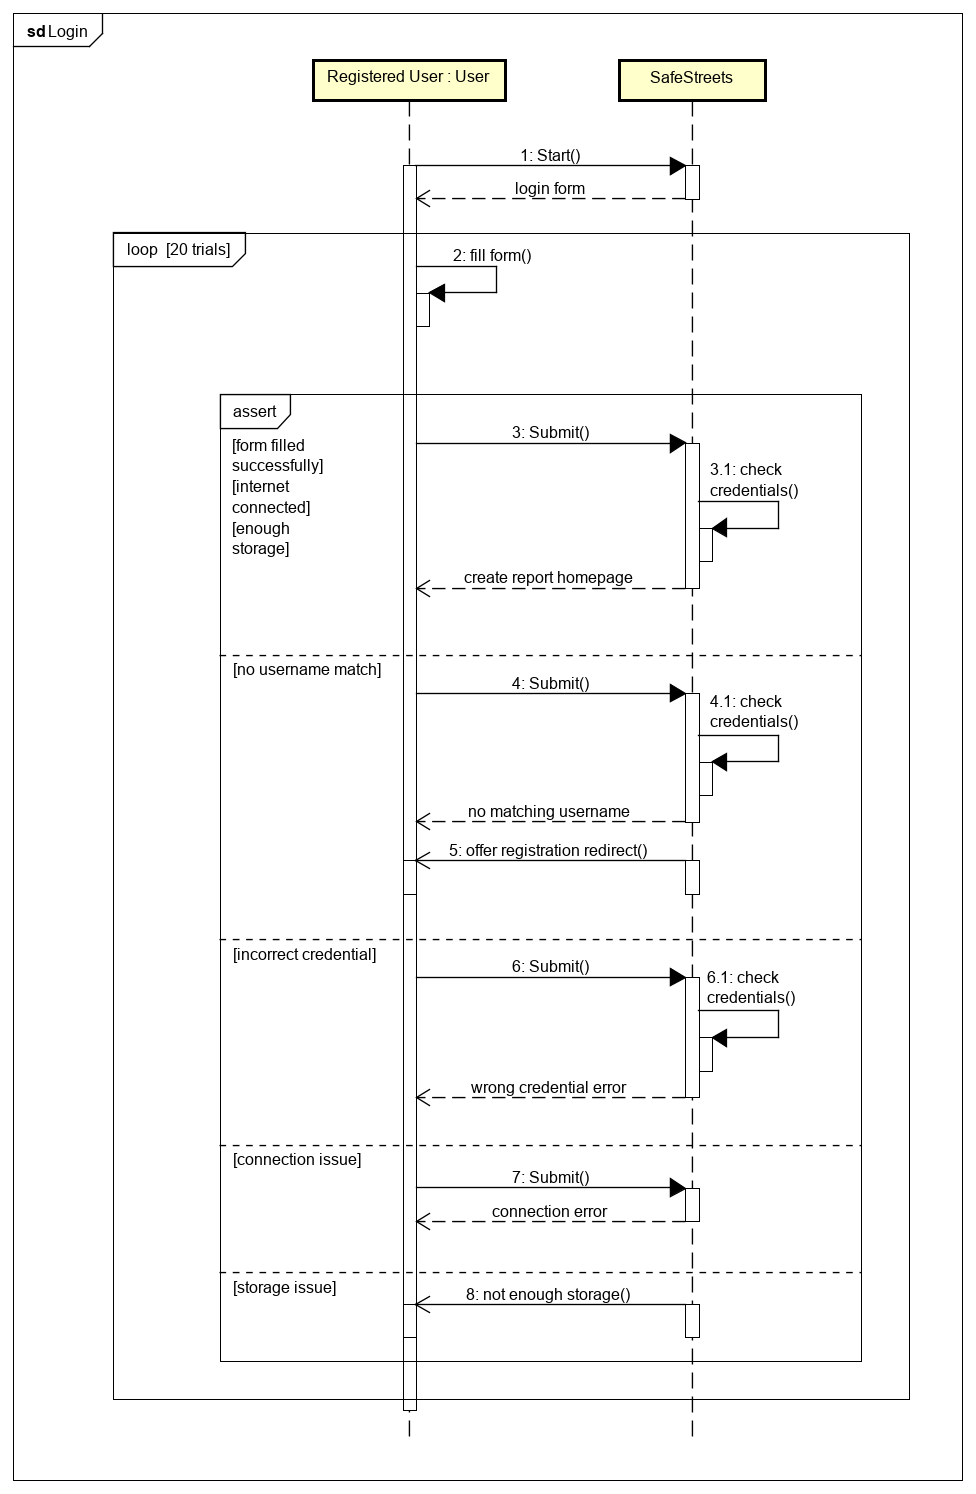
\includegraphics[width=\textwidth, height=0.90\textheight]{login-SD.png}
\end{figure}
%***place holder for login-sd***

\paragraph{Giving Permission}
\hfill \break

\begin{table}[H]
\begin{flushleft}\emph{\textbf{Use Case}}\end{flushleft}
\footnotesize
\centering
\settowidth\tymin{\textbf{Entry conditions}}
\setlength\extrarowheight{2pt}
\begin{tabulary}{\textwidth}{|J|J|}
\hline
Name            & Giving Permission \\
\hline 
Actors          & Registered User \\
\hline 
Entry Condition & The user logged in to the app for the first time \\
\hline 
Event Flow      & 
\begin{minipage}[t]{0.7\textwidth}
\begin{enumerate} 
\item After logging a dialog message asking for access to phone camera appears
\item The user clicks on the ‘accept’ button
\item Dialog message asking for access to location data appears
\item The user clicks on the ‘accept’ button
\end{enumerate}
\end{minipage}\\
\hline

Exit Condition  & The user grants access to both camera and location data \\
\hline 
Exceptions      & 
\begin{minipage}[t]{0.8\textwidth}
\begin{itemize} 
\item The user denies access to either camera or location data: A message appears stating that if access is not granted no trafficviolation reports can be made and asking the user if they want to continue anyway If the user continues, they will not be able to make violation reports If the user grants access, all functions of the system are available to be exploited by the user
\end{itemize}
\end{minipage}\\
\hline
\end{tabulary}
\caption{\label{tab:Usecase-Give-Permission}Usecase for Giving Permission}
\end{table}

After first login, the user is asked to give permission for the application to access the device camera and location services. If the user denies, the they are shown a warning message that they will be unable to make report submission until they accept access.

\begin{figure}[H]
\begin{flushleft}\emph{\textbf{Sequence Diagram}}\end{flushleft}
\caption{Sequence Diagram for Giving Permission}
\label{fig:SD-Give-Permission}
\centering
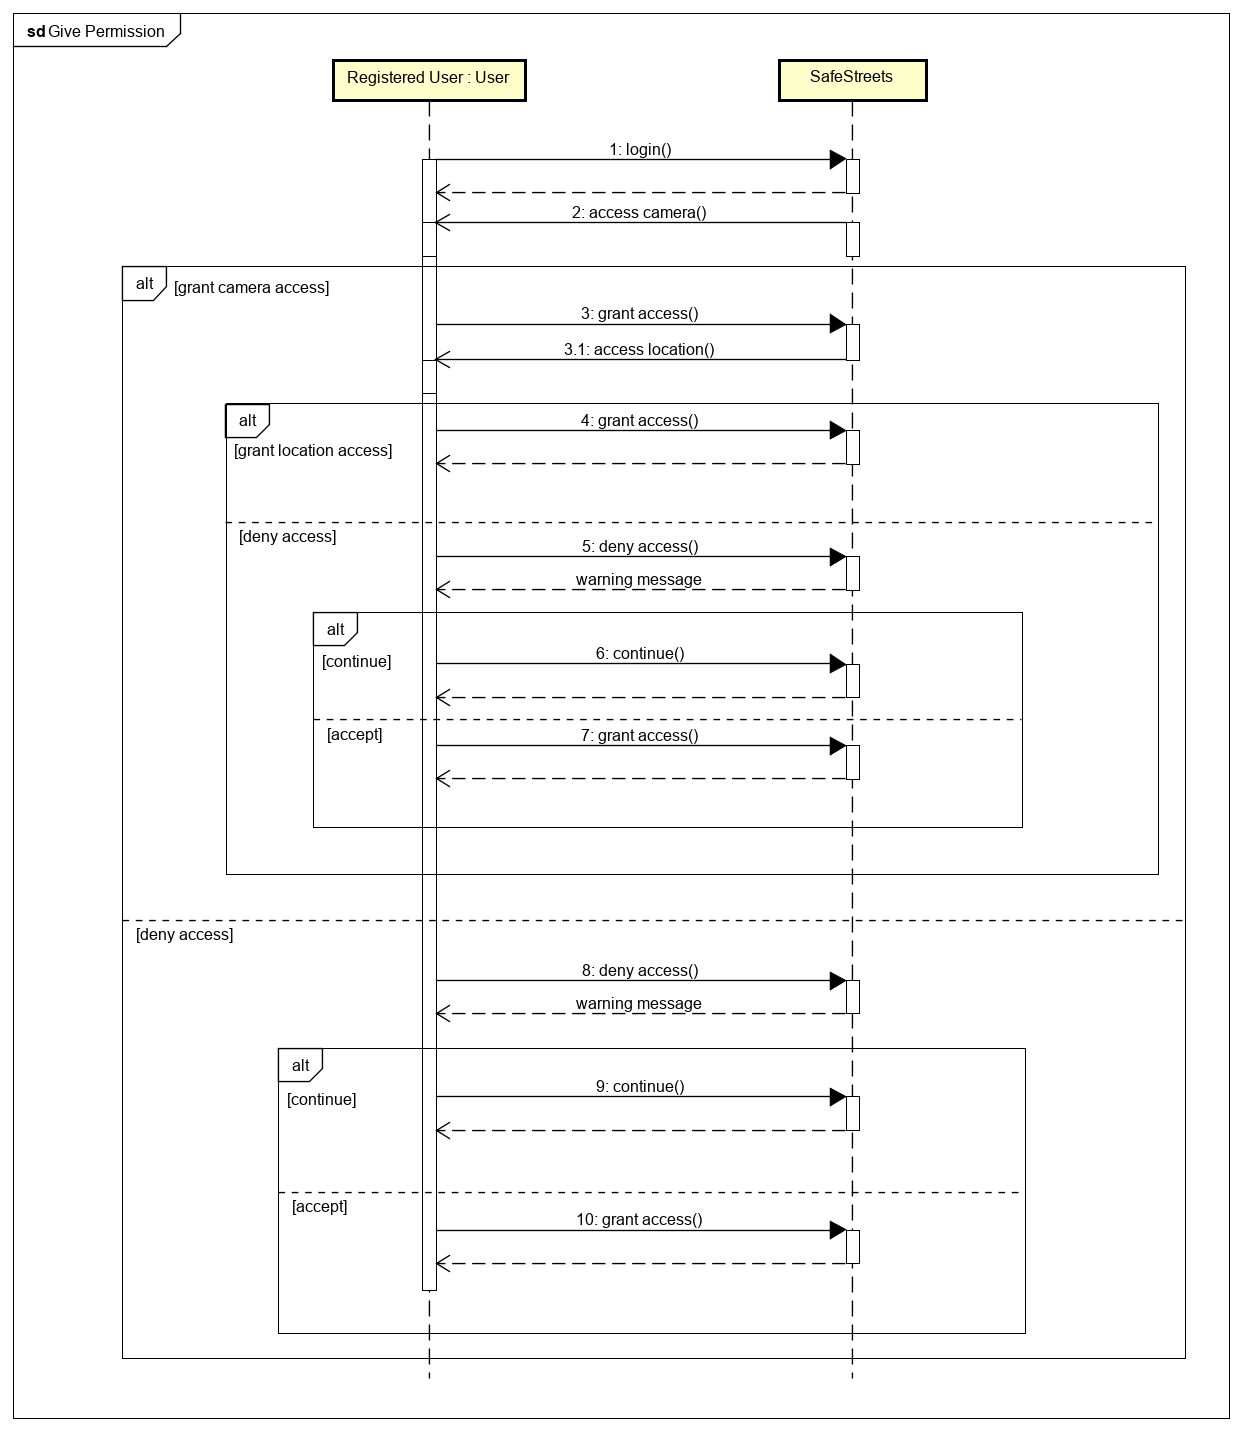
\includegraphics[width=\textwidth, height=0.90\textheight]{give-permission-SD.png}
\end{figure}
%***place holder for give-permission-sd***

\paragraph{View Report History}
\hfill \break



\begin{table}[H]
\begin{flushleft}\emph{\textbf{Use Case}}\end{flushleft}
\footnotesize
\centering
\settowidth\tymin{\textbf{Entry conditions}}
\setlength\extrarowheight{2pt}
\begin{tabulary}{\textwidth}{|J|J|}
\hline
Name             & View Report History \\
\hline 
Actor            & Registered User \\ 
\hline 
Entry conditions & Signed in user wishes to see previously submitted report\\
\hline 
Events flow      & 
\begin{minipage}[t]{0.7\textwidth}
\begin{enumerate} 
\item From the homepage the user opens the view history section
\item The user chooses from a group of filters to apply to history
\item The user is presented with a list of previously submitted reports that match filters
\end{enumerate}
\end{minipage}\\
\hline
Exit conditions  & The user is presented with report history \\
\hline 
Exceptions       & 
\begin{minipage}[t]{0.8\textwidth}
\begin{itemize} 
\item No reports match applied filters: A message is presented stating that there are no matching reports in history
\end{itemize}
\end{minipage}\\
\hline
\end{tabulary}
\caption{\label{tab:Usecase-View-Report-History}Usecase for View Report History}
\end{table}

The last of the general  functions represented in the following figure, is the Report History functionality. Where, the user chooses the filtering criteria and they are presented with the violation reports previously submitted by them that match the search criteria.

%***place holder for view-history-sd***
\begin{figure}[H]
\begin{flushleft}\emph{\textbf{Sequence Diagram}}\end{flushleft}
\caption{Sequence Diagram for View Report History}
\label{fig:SD-View-Report-History}
\centering
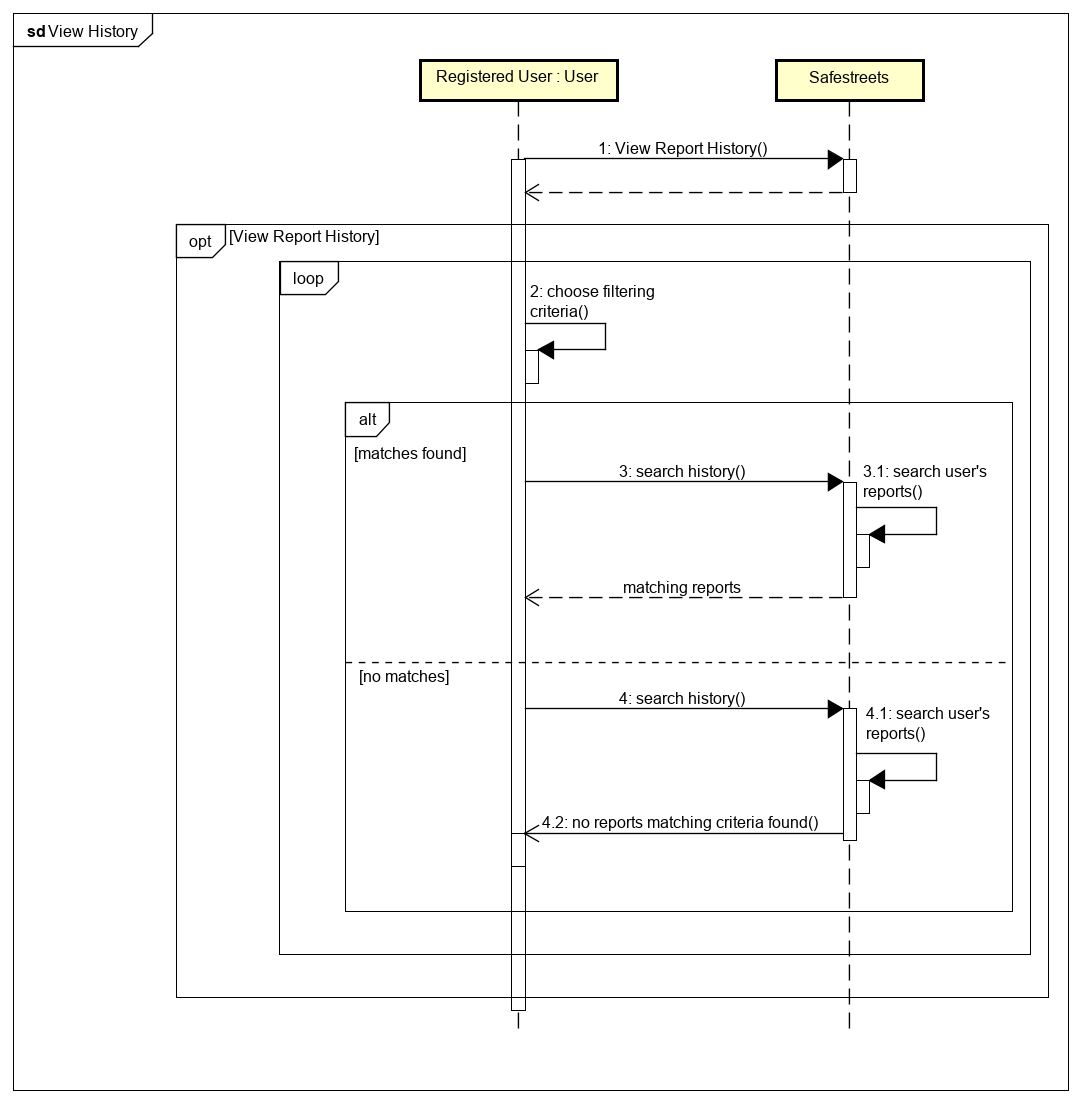
\includegraphics[width=\textwidth, height=0.90\textheight]{view-history-SD.png}
\end{figure}
